\documentclass[tikz,border=5pt]{standalone}
\usepackage{fontspec}
\setmainfont{TeX Gyre Termes}
\setsansfont{TeX Gyre Heros}
\usepackage{pgfplots}
\pgfplotsset{compat=1.18}
\usetikzlibrary{patterns,positioning,arrows.meta}
\definecolor{blue}{HTML}{0072B2}
\definecolor{green}{HTML}{009E73}
\definecolor{orange}{HTML}{E69F00}
\definecolor{red}{HTML}{D55E00}
\definecolor{grey}{HTML}{8D9399}
\pgfplotsset{every axis/.append style={width=8.1cm,height=5.3cm,
font=\small,axis lines=left,axis line style={grey},tick align=outside,
enlarge x limits=.18,ymajorgrids=true,grid style={grey!18},
tick label style={font=\small},label style={font=\small},
nodes near coords style={font=\small,/pgf/number format/fixed,/pgf/number format/precision=2,/pgf/number format/1000 sep={,}},clip=false}}
\begin{document}
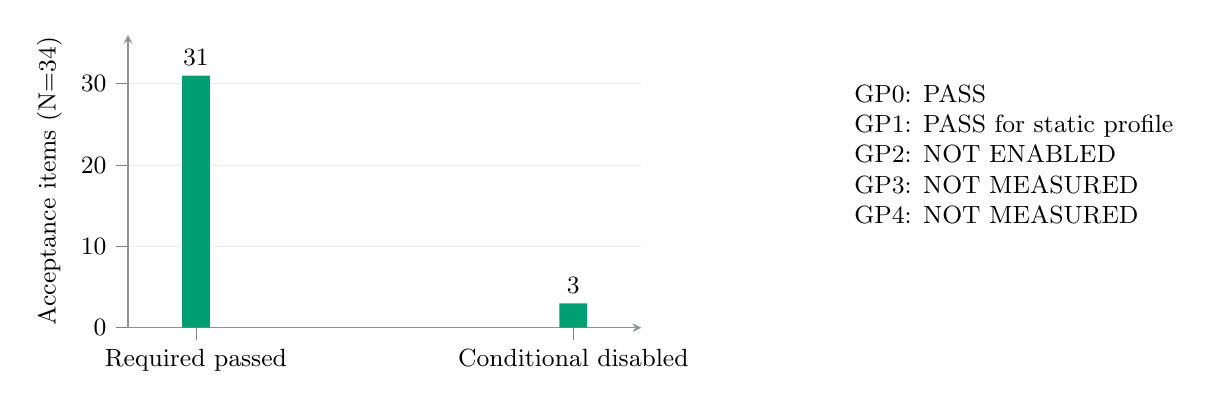
\begin{tikzpicture}
\begin{axis}[ybar,xtick={0,1},xticklabels={Required passed,Conditional disabled},ymin=0,ymax=36,ylabel={Acceptance items (N=34)},nodes near coords]
\addplot[fill=green,draw=none] coordinates {(0,31) (1,3)};

\end{axis}
\node[align=left,anchor=west,font=\small] at (9.1cm,2.2cm) {GP0: PASS\\GP1: PASS for static profile\\GP2: NOT ENABLED\\GP3: NOT MEASURED\\GP4: NOT MEASURED};\end{tikzpicture}
\end{document}
